\chapter{Implementierung}
\label{chp:implementierung}

In diesem Kapitel wird die gesamte Systemumgebung um das Steuerelement in Form eines Raspberry Pi beschrieben und erläutert.


\section{Installation und Konfiguration Raspberry Pi}
\label{sec:inst_konf_raspi}

Die Steuerung des Mars-Rover-Modells erfolgt zentral über einen Raspberry Pi 3 Model B Plus (Revision 1.3).
Auf diesem ist die Debian-basierte Distribution Raspbian for Robots der US-amerikanischen Firma Dexter Industries installiert worden.
Dieses Betriebssystem enthält standardmäßig viele zusätzliche Anwendungen und Treiber vorinstalliert für den Einsatz des Raspberry Pi zur Steuerung von Robotern.
Insbesondere sind alle benötigten Bibliotheken zur Nutzung der zusätzlichen Platine BrickPi vorinstalliert und -konfiguriert.
Der BrickPi ist ebenfalls ein Produkt von Dexter Industries und stellt eine Schnittstelle zwischen den verschiedenen LEGO-Mindstorms-Sensoren und -Motoren zum Raspberry Pi bereit.
Er fungiert dabei auch als Stromquelle für diese sowie für den Raspberry Pi selbst und muss dazu lediglich auf dessen Pins für \acf{gpio} aufgesteckt werden.
Da jeder BrickPi nur über vier Ausgänge zum Betrieb von EV3-Motoren verfügt, ist der gleichzeitige Einsatz von drei BrickPis nötig, um die zehn Motoren des Modells anzutreiben.
Dabei kann jedes der sechs Räder separat durch einen Motor angetrieben sowie die äußeren vier Räder einzeln gelenkt werden.
Eine Lenkung der mittleren Räder ist zum aktuellen Zeitpunkt nicht notwendig, kann aber problemlos über die verbleibenden beiden Ports der BrickPis ergänzt werden, beispielsweise um seitliche Fahrten zu ermöglichen.

\section{Installation und Konfiguration Kamera}
\label{sec:inst_konf_kamera}

Für die Videoeingabe wird die originale Raspberry Pi Camera V2 genutzt.
Diese nutzt den CMOS-Sensor Sony IMX219 mit einer Auflösung von bis zu 8 Megapixeln \cite{pagnutti2017}.
Die Aufnahmen erfolgen mit einer reduzierten Auflösung von $1280 \times 720$ Pixeln, um eine Frequenz von 60 Hz zu ermöglichen. 
So ist sichergestellt, dass Wasserobjekte auch während der Fahrt gut erkannt werden können.


\begin{wrapfigure}{l}{0.25\textwidth}
	\centering
	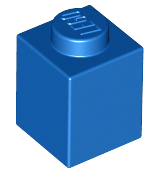
\includegraphics[width=0.9\linewidth]{../Images/3005.png}
	\vspace{0.5em}
	\parbox[c]{0.8\linewidth}{\footnotesize
		\centering
		\vspace{1em}
		Quelle: \url{https://www.bricklink.com/v2/catalog/catalogitem.page?P=3005\&C=7}
	}
	\captionsetup{format=plain}
	\caption{Blauer LEGO-Stein 3005}
	\label{fig:lego3005}
\end{wrapfigure}

Die Objekterkennung für Wasserobjekte erfolgt mithilfe der Programmbibliotheken picamera und OpenCV.
Erstere stellt eine Schnittstelle zwischen der Raspberry-Pi-Kamera und Python zur Verfügung.
Letztere ermöglicht die Echtzeitverarbeitung der Kamerabilder:
Die Objekte werden auf Basis ihrer blauen Farbe erkannt, da sich diese deutlich von der charakteristischen Farbe der Vorbildlandschaften des Mars unterscheidet.
Letztere sei eine \enquote{predominantly yellowish brown color with only subtle variation} \cite{maki1999}.
Die LEGO-Steine, welche als Wasserobjekte fungieren, haben die LEGO-Farb-ID $7$.
Diese korrespondiert mit dem Farbcode \#0057A6 in Hexadezimaldarstellung.
Ein solcher LEGO-Stein ist in Abbildung \ref{fig:lego3005} dargestellt.

Da eine farbwertbasierte Erkennung der Wasserobjekte genutzt wird, entfällt das Trainieren eines Erkennungsalgorithmus, wie es bei einem neuronalen Netz nötig wäre.
Die Farbeigenschaften des LEGO-Steins werden in Komponenten für rote, grüne und blaue Farbanteile aufgeteilt und in der Konfiguration hinterlegt.
Das Python-Skript berechnet für die \acs{rgb}-Farbangaben die entsprechenden \acs{hsv}-Werte.
In letzterer Darstellung ist die Information über tatsächliche Farbe nur noch im Hue-Wert ($0$ bis $255$) hinterlegt, sodass für diesen eine bestimmte Abweichung (Standard: $\pm 10$) definiert werden kann.
Die Sättigung (Saturation) und der Hellwert (Value) (beide ebenfalls von $0$ bis $255$ definiert) werden in einem breiten Spektrum toleriert:
Standardmäßig lässt das Skript hier Werte von mindestens $80$ und höchstens $255$ zu.
Mithilfe dieser Parameter wird eine solide Erkennung der Präsenz der LEGO-Steine gewährleistet.